\chapter{Analisi statiche}
In questa sezione verranno presentati gli strumenti utilizzati per effettuare le scansioni statiche. I risultati verranno aggregati e commentati insieme a quelli delle analisi dinamiche nella sezione $3$.

%----------------------------------------------------%
%--------------------- MARA -------------------------%
%----------------------------------------------------%

\section{MARA Framework}

\begin{figure}[h]
	\centering 
	\fbox{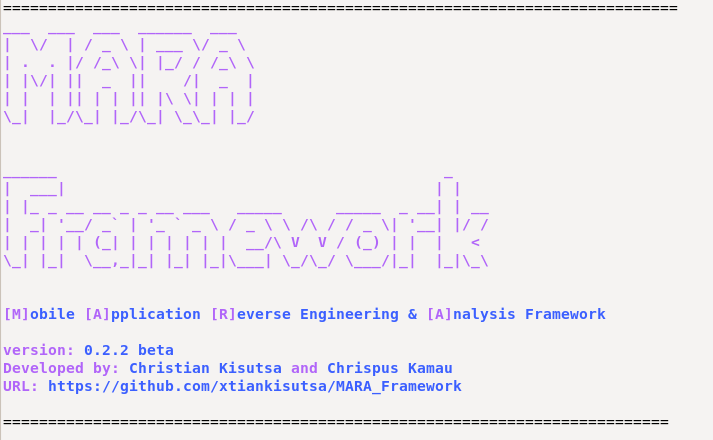
\includegraphics[width=.5\textwidth]{mara/MARABN}}
	\caption{MARA Framework}
	\label{fig:mara} 
\end{figure}

Il primo strumento utilizzato è stato \ac{MARA} Framework(figura \ref{fig:mara})\cite{MARA}. Questo framework unisce vari strumenti comunemente utilizzati per effettuare reverse engineering ed analisi di applicazioni mobili. MARA è particolarmente focalizzato sulle minacce indicate dalla OWASP Foundation\cite{OWASP} come più diffuse e pericolose.
Le operazioni che permette di fare sono le seguenti:
\begin{itemize}
	\item Reverse engineering dell'apk
	\item De-offuscamento dell'apk
	\item Analisi dell'apk
	\item Analisi del manifest
	\item Analisi del codice sorgente
\end{itemize}

L'esecuzione dell'analisi di MARA sull'apk si compone di vari passi (figura \ref{fig:maraScanA}) e si può vedere come si concentri particolarmente sulle vulnerabilità indicate dalla OWASP Foundation.
\begin{figure}[h]
	\centering
	\fbox{
		\subfloat[]{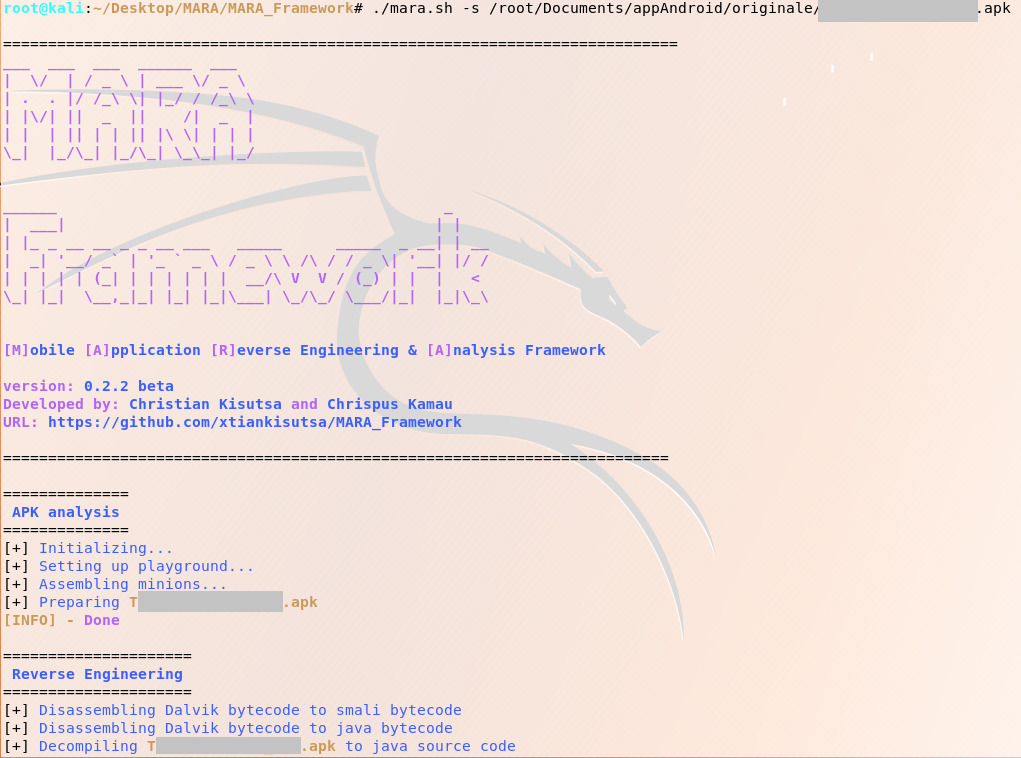
\includegraphics[width=.45\textwidth]{mara/MARAexecution01BN}\label{fig:maraScanA}} \quad
		\subfloat[]{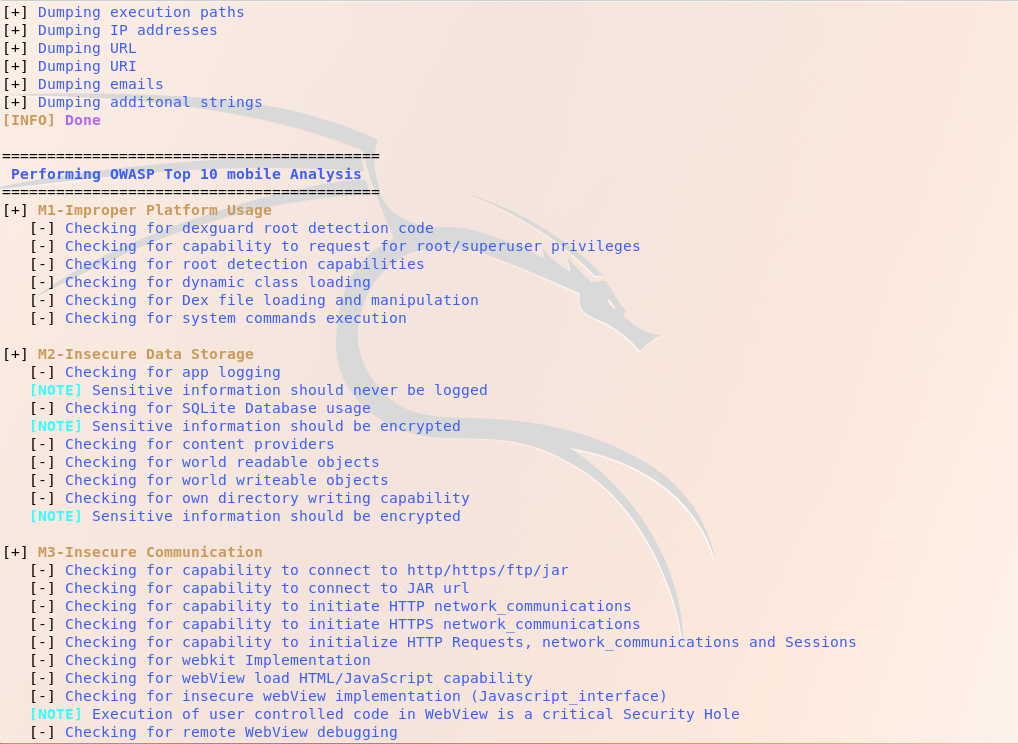
\includegraphics[width=.45\textwidth]{mara/MARAexecution03BN}\label{fig:maraScanB}}
	}
	\caption{Alcune delle operazioni effettuate da MARA.}
\end{figure}

Il primo passo effettuato è il reverse engineering dell'apk. Al suo interno, MARA ha a disposizione strumenti come \emph{apktool}, \emph{baksmali}, \emph{enjarify} e \emph{jadx}, in grado di ricavare il codice sorgente partendo dall'apk. Come si può vedere dalla figura \ref{fig:source}, è stato effettivamente ottenuto il codice sorgente dell'applicazione che può essere analizzato tramite strumenti automatici (lo stesso MARA lo fa) o manualmente.

\begin{figure}[h]
	\centering 
	\fbox{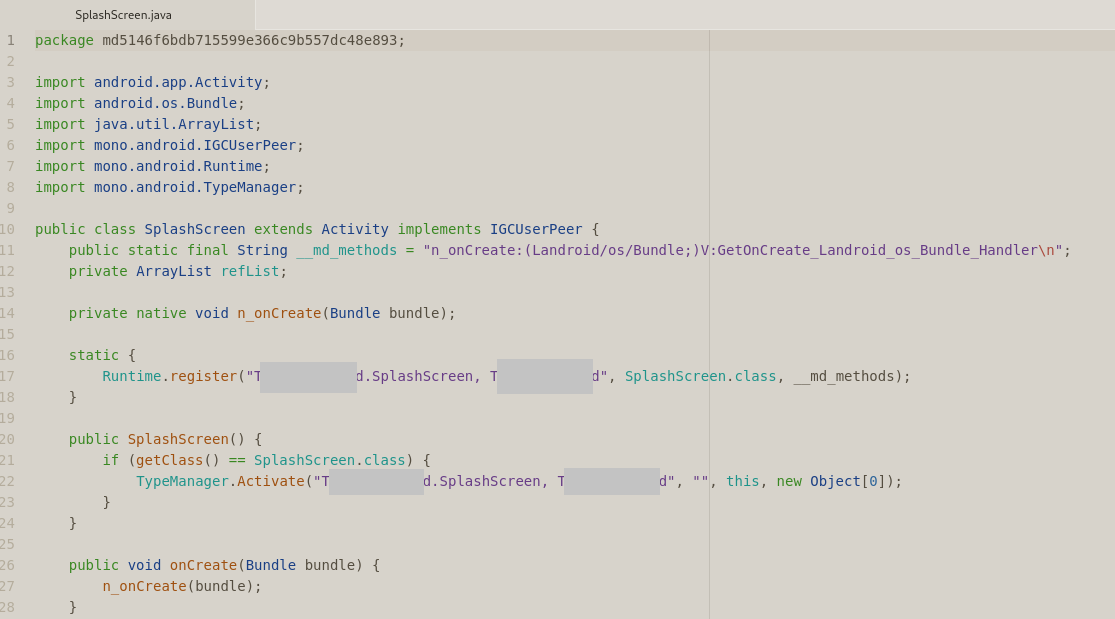
\includegraphics[width=.95\textwidth]{reverse/sourceBN2}} 
	\caption{Codice sorgente ottenuto.}
	\label{fig:source} 
\end{figure}

Successivamente si passa all'analisi del manifest, controllando activities, receivers e services eventualmente esportati. Vengono verificati i permessi ed altre opzioni ritenute pericolose o compromettenti (backup, debug, ecc.). Vengono estratti e controllati i certificati ed analizzato il codice sorgente alla ricerca di bug o comportamenti malevoli. Dopo queste verifiche preliminari, vengono eseguiti i controlli principali su cui si basa MARA; l'OWASP top 10 mobile (figura \ref{fig:maraScanB}). Come ultimo passo, vengono effettuati altri controlli standard come l'utilizzo di primitive crittografiche obsolete, utilizzo di connessioni non sicure, ecc.

%----------------------------------------------------%
%-------------------- SUPER -------------------------%
%----------------------------------------------------%

\section{SUPER Android Analyzer}

Il secondo strumento utilizzato è stato \ac{SUPER} Android Analyzer (figura \ref{fig:super}) \cite{SUPER}. 

\begin{figure}[h]
	\centering 
	
\includegraphics[width=.2\textwidth]{super/super} 
	\caption{SUPER logo.}
	\label{fig:super} 
\end{figure}

SUPER è un'applicazione a riga di comando, scritta in linguaggio Rust, che analizza files di tipo apk in cerca di vulnerabilità. È in grado di effettuare il reverse engineering dell'apk ed applicare una serie di regole per determinare l'effettiva presenza di vulnerabilità all'interno dell'applicazione. 

La particolarità di RUST è la sua estrema estensibilità. Tutte le regole sono infatti memorizzate in un file (\emph{rules.json}) ed è sempre possibile modificare quelle esistenti o crearne di nuove. Un esempio di regola potrebbe essere la seguente:

\lstinputlisting[caption=Esempio di regola SUPER]{code/super.json}

Utilizzando questa regola, se viene trovata una porzione di codice che rispecchia il valore nel campo \emph{regex} e viene garantito il permesso specificato nel campo \emph{permissions} (in questo caso WRITE EXTERNAL STORAGE), allora viene rilevata una vulnerabilità con livello di criticità \emph{high} (campo \emph{criticality}) e viene fornita la descrizione presente nel campo \emph{description}.

\begin{figure}[h]
	\centering 
	\fbox{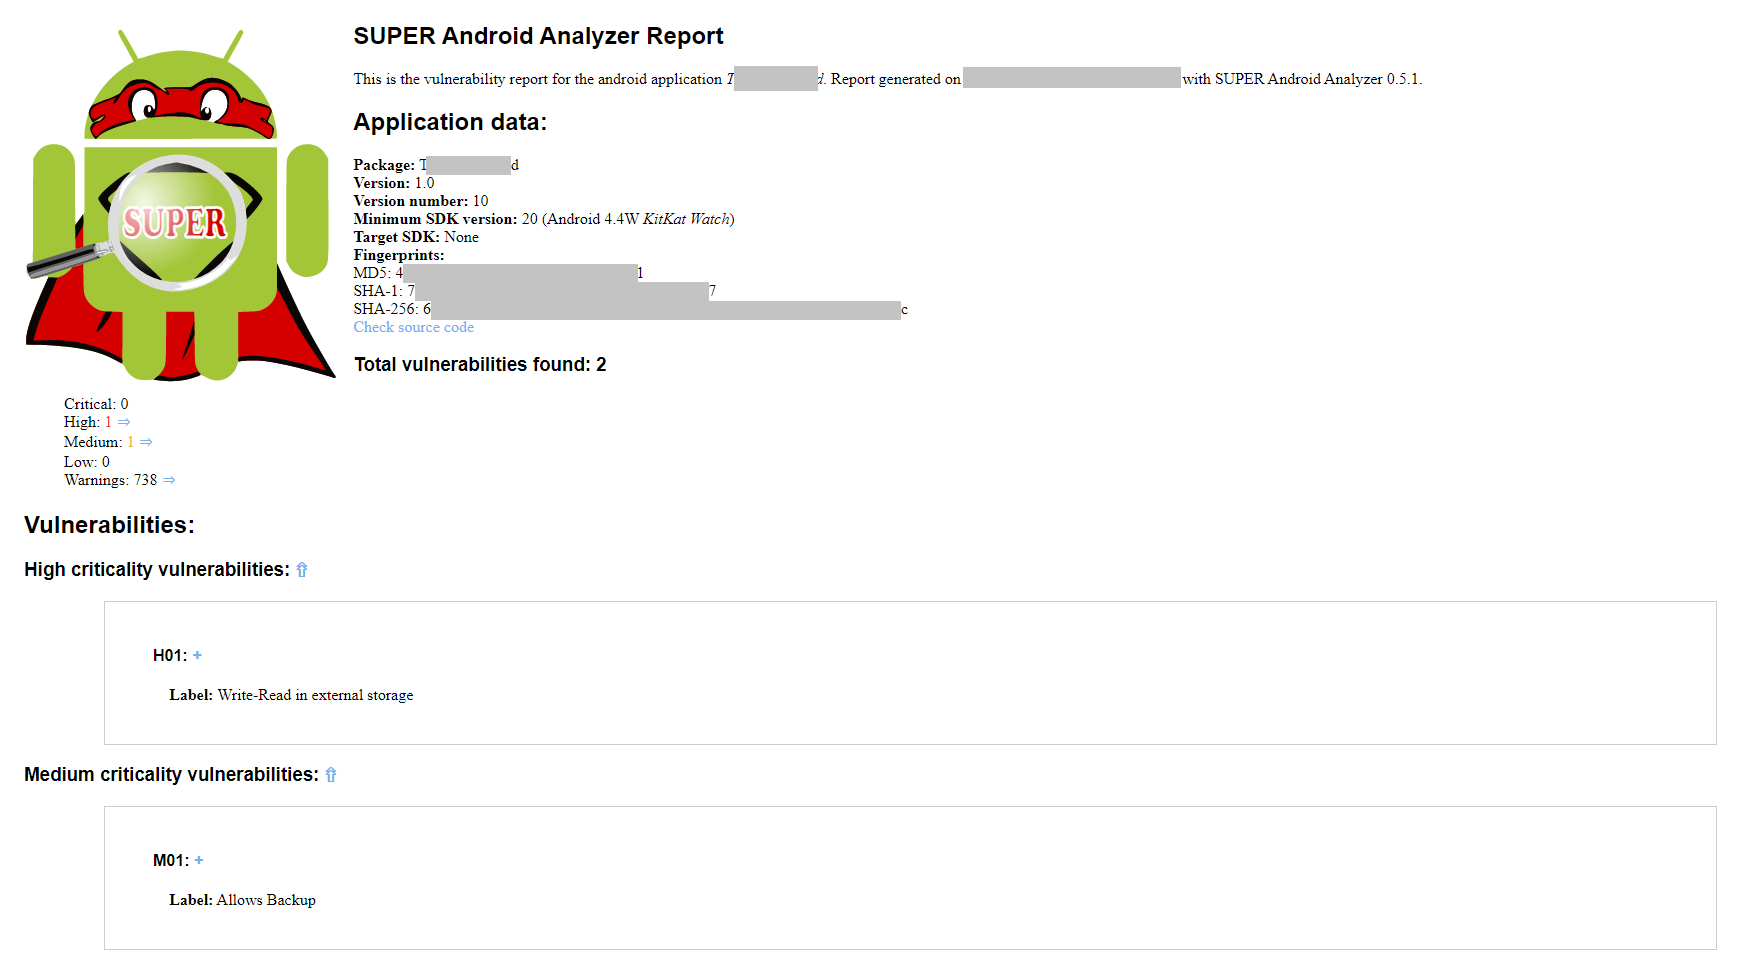
\includegraphics[width=.9\textwidth]{super/superResults}}
	\caption{Report di SUPER}
	\label{fig:superResults} 
\end{figure}

La scansione con SUPER genera un file html (figura \ref{fig:superResults}) nel quale, oltre a trovare informazioni di base sull'applicazione, è presente la lista delle vulnerabilità riscontrate che in questo caso sono una di livello alto ed una di livello medio. Espandendo la sezione relativa ad ogni vulnerabilità presente nel report, viene riportata la porzione di codice affetta dalla stessa (figura \ref{fig:superVuln}). 

\begin{figure}[h]
	\centering 
	\fbox{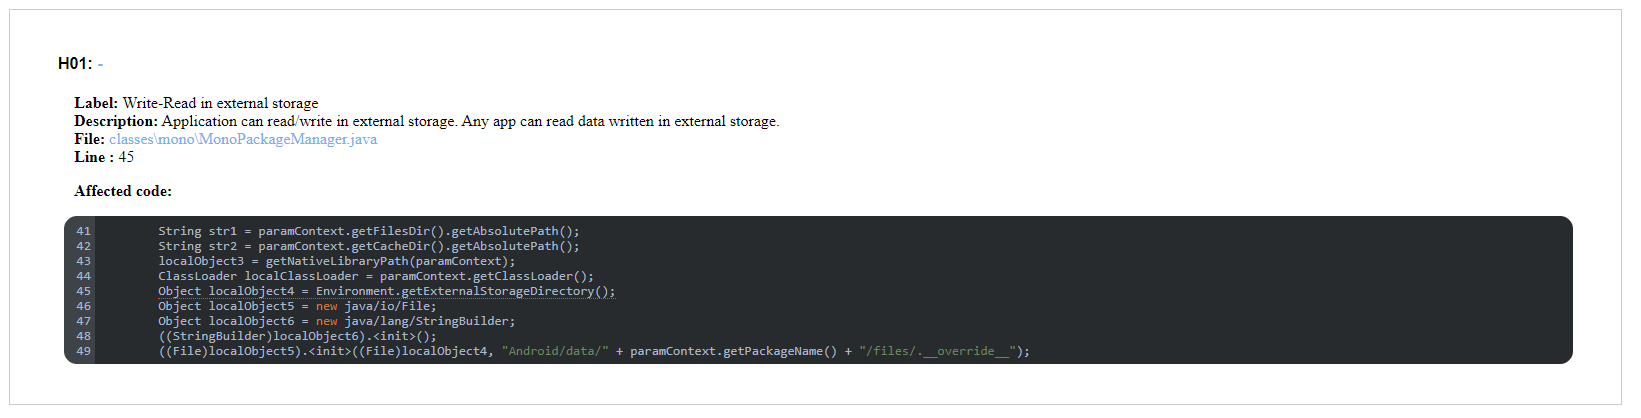
\includegraphics[width=.9\textwidth]{super/superVuln}} 
	\caption{Porzione di codice affetta dalla vulnerabilità}
	\label{fig:superVuln} 
\end{figure}

%----------------------------------------------------%
%--------------------- QARK -------------------------%
%----------------------------------------------------%

\section{QARK}
\begin{figure}[h]
	\centering 
	\fbox{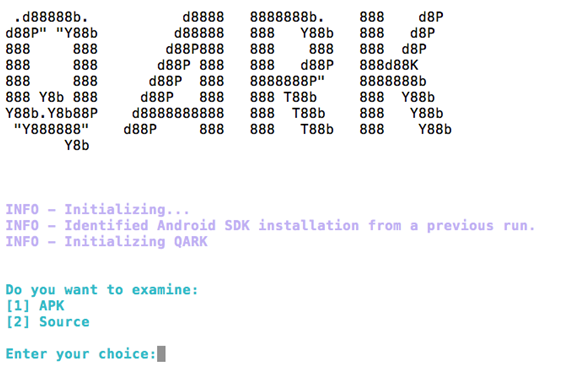
\includegraphics[width=.45\textwidth]{qark/QARK}}
	\caption{QARK}
	\label{fig:qark}
\end{figure}

L'ultimo strumento utilizzato è stato \ac{QARK} \cite{QARK} (figura \ref{fig:qark}). Le vulnerabilità sulle quali si concentra maggiormente sono le seguenti:
\begin{itemize}
	\item Componenti esportati inavvertitamente
	\item Intent vulnerabili ad intercettazioni
	\item Scorretta validazione dei certificati X.$509$
	\item Creazione di files world-readable o world-writeable
	\item Attività che possono far filtrare informazioni
	\item Utilizzo di Intent sticky
	\item Invio non sicuro di Broadcast Intents
	\item Informazioni hard-coded all'interno del codice
	\item Configurazioni potenzialmente vulnerabili delle WebView
	\item Tapjacking
	\item Applicazioni che abilitano il backup
	\item Applicazioni debuggabili
	\item Supporto ad API non aggiornate o con vulnerabilità note
\end{itemize}

La particolarità che contraddistingue QARK è la possibilità di generare comandi \ac{ADB} o interi apk in grado di sfruttare alcune delle vulnerabilità rilevate.

Il risultato dell'analisi di QARK, viene fornito tramite un file html (figura \ref{fig:qarkResults}) contenente l'elenco dei singoli problemi rilevati, la relativa descrizione e il file che li origina.
\begin{figure}[h]
	\centering 
	\fbox{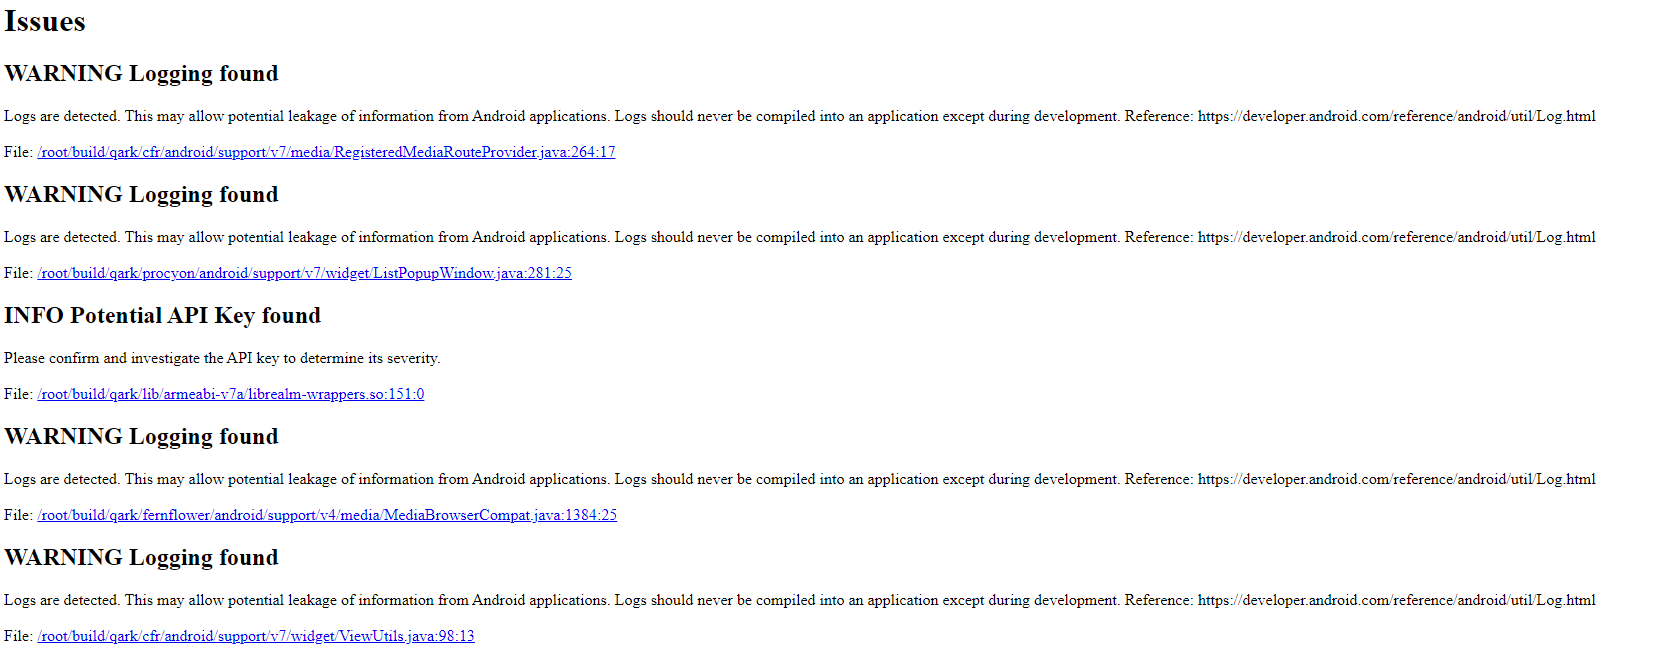
\includegraphics[width=.9\textwidth]{qark/QARKresults}}
	\caption{Risultati forniti dalla scansione di QARK.}
	\label{fig:qarkResults}
\end{figure}